%! Author = joels
%! Date = 05/01/2021

\section{Grundkonzepte}
Apps bestehen aus lose gekoppelten, wiederverwendbaren Komponenten (Activities, Content Providers, Services \& Broadcast receivers).\\
Android hat die Kontrolle über ausgeführte Apps:
\begin{itemize}[topsep=0pt, leftmargin=4mm]
    \setlength\itemsep{-0.3em}
    \item Verwaltung des Lebenszyklus
    \item Kommunikation zwischen Komponenten
    \item Terminierung bei Bedarf (z.B. Speicherknappheit)
\end{itemize}
\subsection{Activities}
Beim App-Start wird die Main Activity von Android erzeugt und ausgeführt. Activities besitzen eine grafische Obefläche und verarbeiten Benutzereingaben.
\begin{lstlisting}
public class MainActivity extends Activity {
    @Override
    protected void onCreate(Bundle savedInstanceState) {
        super.onCreate(savedInstanceState);
        setContentView(R.layout.activity_main);
    }
}
\end{lstlisting}
\textbf{\textcolor{blue}{Activity Lebenszyklus \& Zustände:}}\\
Android ruft beim Zustandwechsel Callback-Methoden auf der Activity auf. Diese Methoden können überschrieben werden.
\begin{center}
    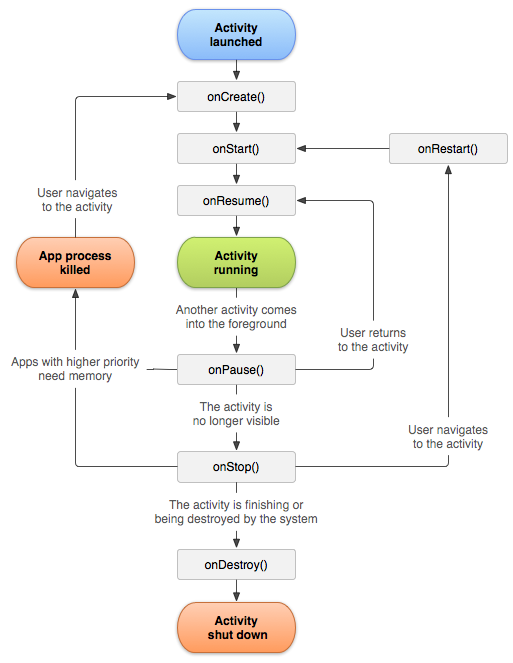
\includegraphics[width=0.7\linewidth]{activity_lebenszyklus.png}
\end{center}
\subsubsection{Anwendungsfälle}
\begin{itemize}[topsep=0pt, leftmargin=4mm]
    \setlength\itemsep{-0.3em}
    \item Erzeugung des GUI: \textcolor{blue}{onCreate()}
    \item Datensicherun: \textcolor{blue}{onPause} für schnelle Operationen, ansonsten \textcolor{blue}{onStop()}
    \item Dienste wie Lokalisierung aktivieren/deaktivieren: \textcolor{blue}{onResume()} und \textcolor{blue}{onPause()}
    \item Zustand des GUI erhalten, z.B. bei Rotation: \textcolor{blue}{onSaveInstanceState()} und \textcolor{blue}{onRestoreInstanceState()}
\end{itemize}
\subsection{Intents}
\begin{itemize}[topsep=0pt, leftmargin=4mm]
    \setlength\itemsep{-0.3em}
    \item Die Kommunikation zwischen Komponenten erfolgt über Intents (Absicht, Vorhaben)
    \item Zwei Arten von Intents:
    \begin{itemize}[topsep=0pt, leftmargin=4mm]
        \setlength\itemsep{-0.3em}
        \item \textcolor{blue}{Explizit:} Aufruf einer definierten Komponente (typischerweise für Komponenten der eigenen App)
        \item \textcolor{blue}{Implizit:} Aufruf einer passenden Komponente (typischerweise für Komponenten aus anderen Apps)
    \end{itemize}
    \item Apps können sich im Android Manifest mit Intent Filters auf implizite Intents registrieren
    \item Intents werden stets von Android verarbeitet
\end{itemize}
\begin{lstlisting}
// Expliziter Intent
Intent secondActivityIntent = new Intent(this, SecondActivity.class);
startActivity(secondActivityIntent);
// Impliziter Intent
Intent sendIntent = new Intent();
sendIntent.setAction(Intent.ACTION_SEND);
sendIntent.setType("text/plain");
sendIntent.putExtra(Intent.EXTRA_TEXT, "Hey!");
startActivity(sendIntent);
\end{lstlisting}
\subsubsection{Beispiel}
\begin{lstlisting}
Button button = findViewById(R.id.buttonNavigate);
button.setOnClickListener(v -> {
    //Explizit
    Intent secondActivityIntent = new Intent(this, SecondActivity.class);
    startActivity(secondActivityIntent);
    //Implizit
    Intent intent = new Intent(Intent.ACTION_VIEW, Uri.parse("http://www.ost.ch"));
    startActivity(intent);
});
\end{lstlisting}
\subsection{Intents mit Parametern}
Zusätzliche Parameter können als Key-Value Paar (Bundle) mit \textcolor{blue}{putExtra()/putExtras()} übergeben werden.
\begin{lstlisting}
// MainActivity.java
Intent intent = new Intent(this, SecondActivity.class);
intent.putExtra("myKey", 42);
startActivity(intent);
// SecondActivity.java
Intent intent = this.getIntent();
String parameter = intent.getStringExtra("key");
\end{lstlisting}
\subsubsection{Hinweise}
\textbf{Mit Intents startet man andere Activities.}\\
$\rightarrow$ Ohne Rückgabewert: \textcolor{blue}{startActivity(Intent)}\\
$\rightarrow$ Mit Rückgabewert: \textcolor{blue}{startActivityForResult(Intent, int)}\\
\textbf{Implizite Intents müssen nicht immer einen Empfänger haben.}\\
$\rightarrow$ Darum immer überprüfen ob Intent einen Empfänger hat:
\begin{lstlisting}
//MainActivity.java
if(intent.resolveActivity(getPackageManager()) != null){
    startActivity(intent);
}
//AndroidManifest.xml
<uses-permission android:name="android.permission.QUERY_ALL_PACKAGES" />
\end{lstlisting}
\subsection{Back Stack (Task)}
\begin{itemize}[topsep=0pt, leftmargin=4mm]
    \setlength\itemsep{-0.3em}
    \item Activities werden im Back-Stack verwaltet
    \item Activities eines Stacks können zu verschiedenen Apps gehören
    \item Dieselbe Activity kann mehrfach im selben Stack enthalten sein
\end{itemize}
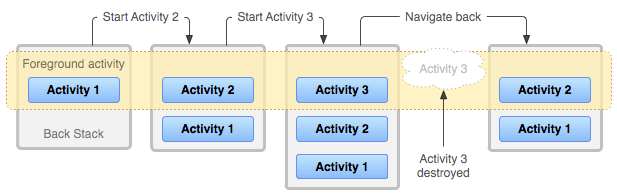
\includegraphics{backstack.png}
\textbf{Ein Back Stack wird auch Task genannt.} Android verwaltet die Ausführung von Tasks. Bei Bedarf können Activities in neuen Tasks gestartet werden.
\subsection{Tasks, Prozesse und Threads}
\begin{itemize}[topsep=0pt, leftmargin=4mm]
    \setlength\itemsep{-0.3em}
    \item Alle Teile eines Apps werden in einer APK-Datei ausgeliefert
    \item Jedes APK wird mit einem eigenen Linux User installiert (Sandbox)
    \item Jedes APK wird in einem eigenen Linux Prozess ausgeführt
    \item Jeder Prozess hat mindestens einen Thread (Main Thread)
\end{itemize}
\subsubsection{Main-Thread}
\begin{itemize}[topsep=0pt, leftmargin=4mm]
    \setlength\itemsep{-0.3em}
    \item Automatisch erzeugt beim Start einer Applikation
    \item Blockierung des Main Threads führt zum ANR-Screen (Application Not Responding)
    \item Langlaufende Operationen immer in eigenen Threads ausführen (Runnable)
    \item \textbf{Achtung:} Nur der Main Thread darf das GUI aktualisieren, sonst Exception
\end{itemize}
\subsection{GUI}
Das GUI kann auf zwei Arten erstellt werden: \textcolor{blue}{Deklarativ} (Beschreibung in XML) und \textcolor{blue}{Imperativ} (Beschreibung im Quellcode).
\subsection{Event Handling}
Listener reagieren auf GUI-Ereignisse und werden bei GUI-Objekt registriert
\begin{lstlisting}
final TextView textView = this.findViewById(R.id.text_example);
Button button = this.findViewById(R.id.button_example);
button.setOnClickListener(new View.OnClickListener() {
    @Override
    public void onClick(View view) {
        textView.setText("Button pressed");
    }
});
// Lambda
button.setOnClickListener(v -> { ... });
// XML
android:onClick="onExampleButtonClicked"
public void onExampleButtonClicked(View view)
\end{lstlisting}
\subsection{Resources}
Alle Dateien, die keinen Code enthalten, werden als Resources bezeichnet. colors.xml für Farbwerte, dimens.xml für Dimensionen, strings.xml für Texte, styles.xml für Styles. Veränderliche Werte
immer in passenden Files definieren und referenzieren. Der Zugriff erfolgt jeweils über die \textcolor{blue}{Resource ID}. $\rightarrow$ Zugriff via \textbf{R-Klasse}
\subsection{Dimensionen}
Android erlaubt die Verwendung folgender Dimensionen:
\begin{itemize}[topsep=0pt, leftmargin=4mm]
    \setlength\itemsep{-0.3em}
    \item dp: Density-independent Pixels
    \item sp: Scale-independent Pixels
    \item px: Pixel
    \item pt: Punkte (1/72 eines physikalischen)
    \item in: Inch
    \item mm: Millimeter
\end{itemize}
\textbf{Empfehlung:} Für Schriften immer in \textcolor{blue}{sp}, Alles andere in \textcolor{blue}{dp}
\subsection{Qualifier}
Resources können in unterschiedlichen Varianten hinterlegt werden:
\begin{itemize}[topsep=0pt, leftmargin=4mm]
    \setlength\itemsep{-0.3em}
    \item Texte für verschiedenen Sprachen
    \item Bilder für verschiedenen Auflösungen
    \item Layouts für unterschiedliche Gerätetypen
\end{itemize}
\subsubsection{Mehrsprachigkeit}
Kein Hardcoded Text sondern über String resource file. Mehrere values Ordner (values\_en, etc.) mit strings.xml Dateien anlegen.
\subsection{App Manifest}
Das AndroidManifest.xml enthält essenzielle Informationen zur App.
\begin{itemize}[topsep=0pt, leftmargin=4mm]
    \setlength\itemsep{-0.3em}
    \item ID, Name, Version und Logo
    \item Enthaltene Komponenten
    \item Hard- und Softwareanforderungen
    \item Benötigte Berechtigungen
\end{itemize}
\subsubsection{Application ID und Version}
\textbf{package:} Eindeutige Identifikation der App, Definiert Namespace, Reversed Internet Domain Format (ch.ost.rj.helloworld)\\
\textbf{versionName:} Ein menschenlesbarer String, Typischerweise Semantic Versioning\\
\textbf{versionCode:} Ein positiver Integer für interne Verwendung, Je höher die Zahl, desto \dq neuer\dq die App, Unterschiedliche Ansätze zur Inkrementierung
\subsubsection{Application-Element}
\begin{itemize}[topsep=0pt, leftmargin=4mm]
    \setlength\itemsep{-0.3em}
    \item Parent der Komponenten ist der Application-Knoten
    \item Application ist auch eine Klasse, die den globalen Zustand der App hält
    \item Eigene Ableitung von Application kann registriert werden
    \item Application enthält LifeCycle-Methoden, die überschrieben werden können
\end{itemize}
\subsubsection{API Level}
\begin{itemize}[topsep=0pt, leftmargin=4mm]
    \setlength\itemsep{-0.3em}
    \item minSdkVersion gibt an, welche Version das Gerät mindestens haben muss
    \item maxSdkVersion gibt an, welche Version das Gerät maximal haben darf
    \item targetSdkVersion ist die Version, welche die App bei der Ausführung verwendet
    \item compileSdkVersion gibt an, mit welcher API das App kompiliert wird
\end{itemize}